\documentclass{article}
\usepackage[utf8]{inputenc}
\usepackage[top=1in, bottom=1in, left=1in, right=1in]{geometry}
\usepackage{indentfirst}
\usepackage{graphicx}
    \DeclareGraphicsExtensions{.png, .jpeg}

\title{CS791m: A2}
\author{Terence Henriod}
\date{\today}

\begin{document}

\maketitle

% \begin{abstract}
An introductory foray into HCI research. Five participants were used to participate in phrase guessing and simple reaction tasks.
% \end{abstract}

\newpage
\subsection{Participants and Experimental Setting}
There were Five (5) participants used in both exercises. Participants ranged in age from $24$ to $72$, with educations from high-school only to college master's degrees. Two participants were male, three were female. For four of the participants, they completed the tasks in a bedroom with a desk and a kneeling chair, with casual conversation occurring outside the room. For the fifth participant, they completed the tasks in a laboratory with causal conversation going on around them. Participants completed all experimental tasks in one sitting.

%
\section{Exercise 2-3}
Conduct a small experiment on redundancy and entropy in written English, similar to Shannon's letter guessing experiment described earlier (see Figure 2.22). Use [3+] participants. For the experiment, use the \texttt{LetterGuessExperiment} software provided on this book's website. Use five trials (phrases) for each participant. \dots Analyze the results for number of letters correctly guessed (redundancy) and the number incorrectly guessed (entropy). Examine the results overall and by participants. Investigate, as well, whether the responses differ according to the position of letters in words and in phrases. Write a brief report on your findings.

%
\subsection{Redundancy vs. Entropy}
\begin{figure}[h!]
\centering
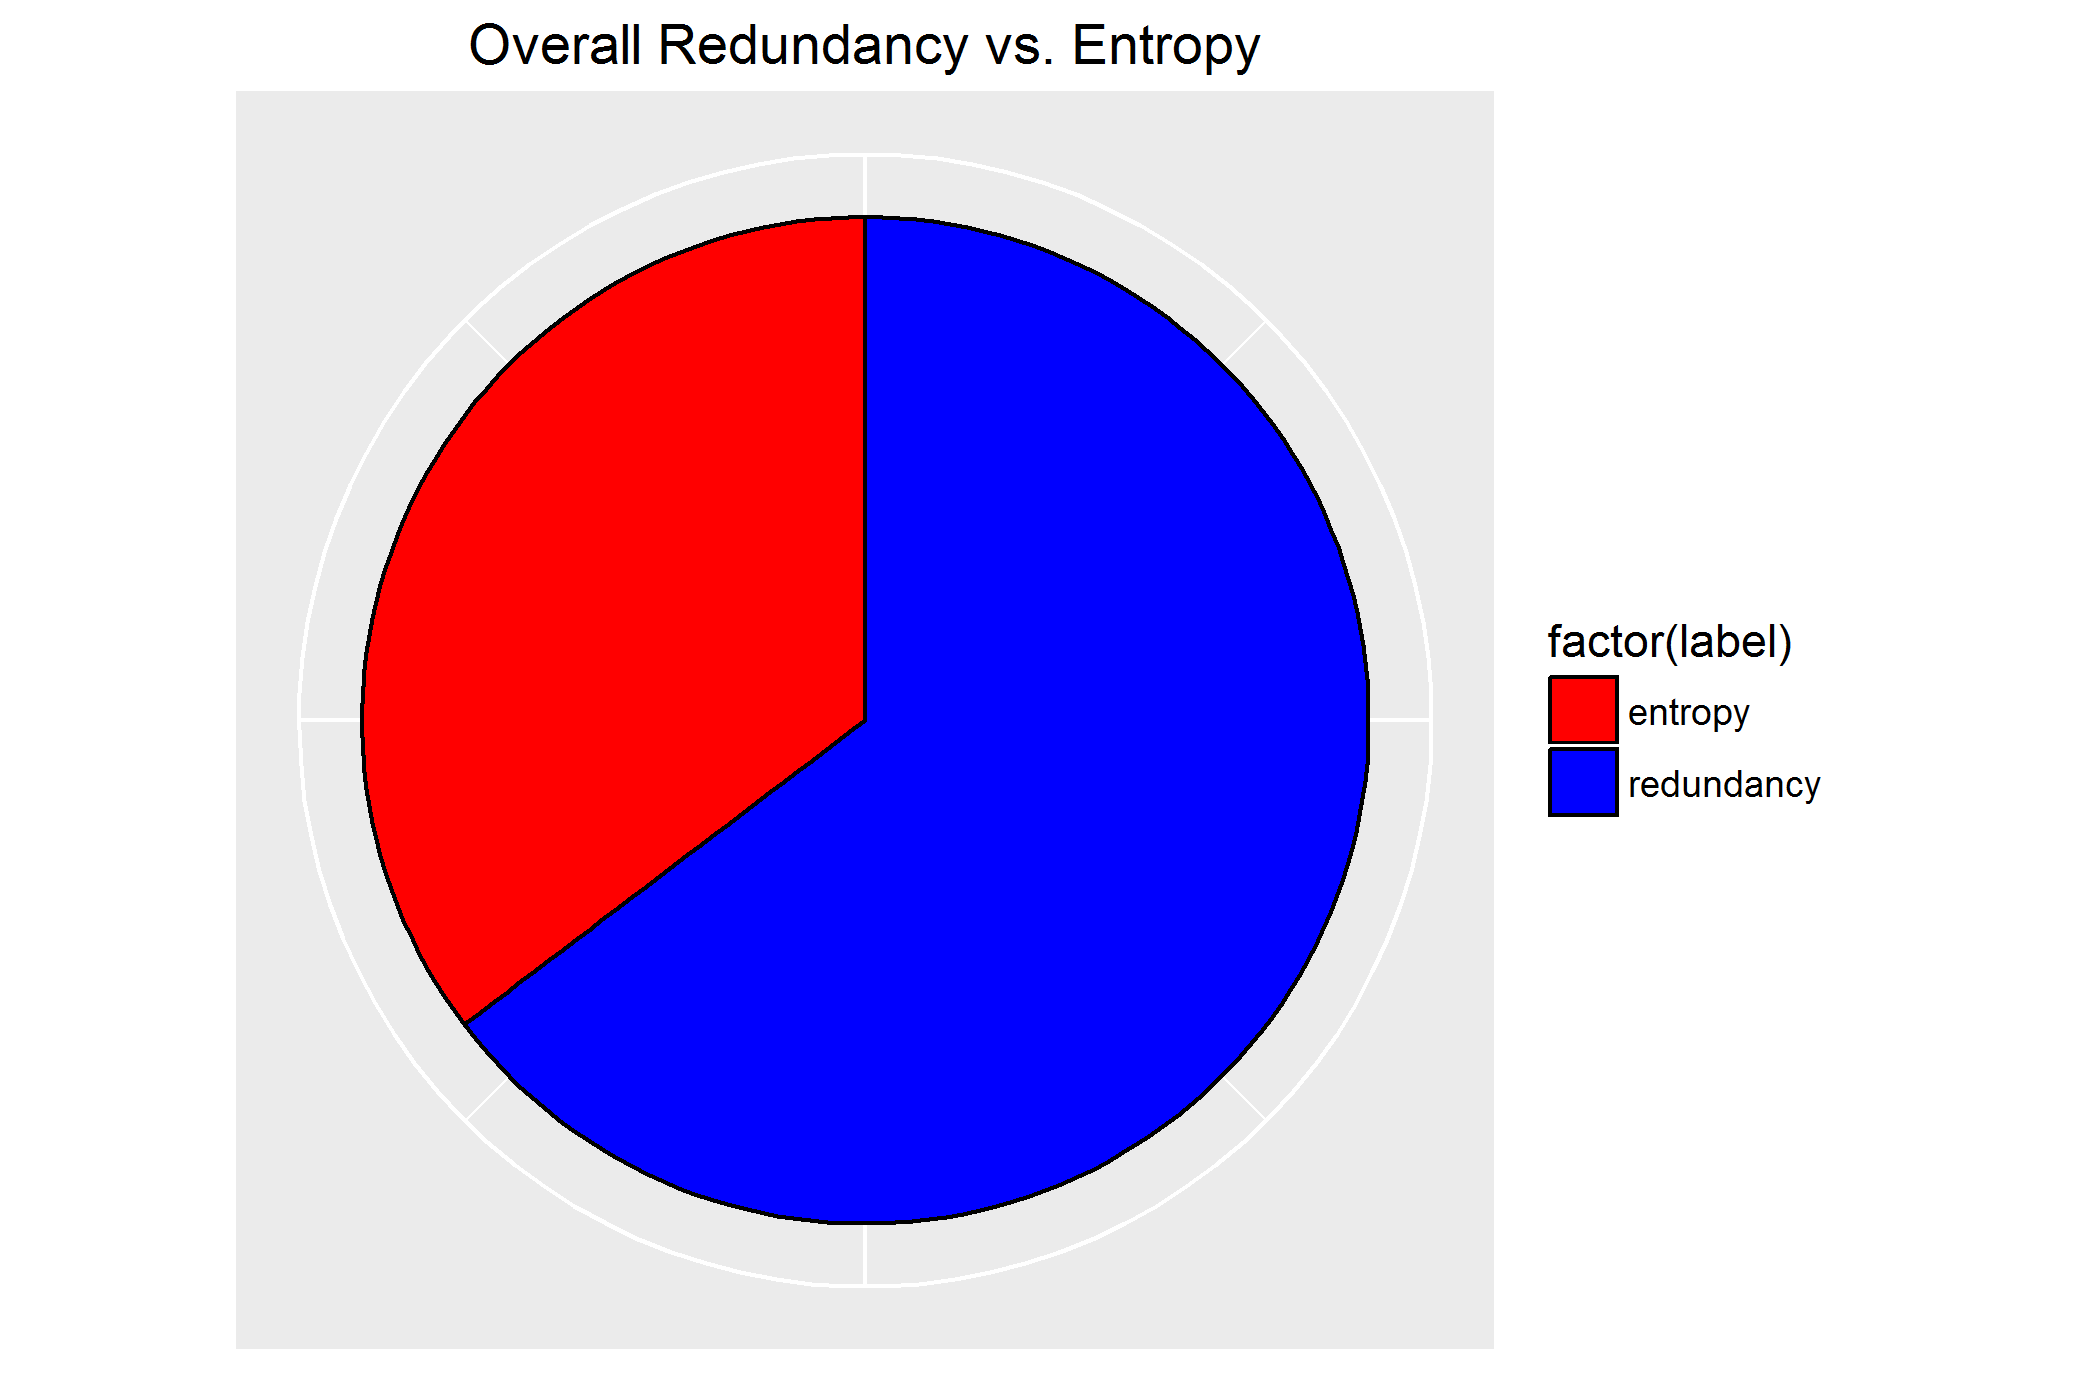
\includegraphics[width=.5\linewidth]{overall-redundancy-entropy}
\caption{A comparison of the overall correct vs. incorrect letter guesses.}
\label{fig:overall-redundancy-entropy}
\end{figure}

\begin{figure}[h!]
\centering
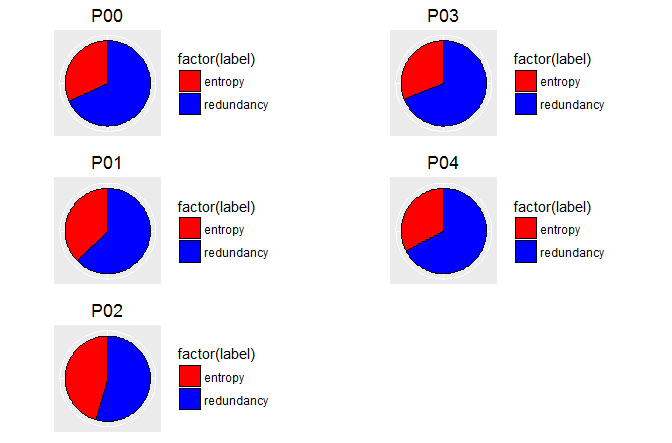
\includegraphics[width=.65\linewidth]{participant-redundancy-entropy}
\caption{A breakdown of correct vs. incorrect guesses by participant.}
\label{fig:participant-redundancy-entropy}
\end{figure}

In general, it appears that participants were able to guess the letter in the phrase correctly more often than not. In fact, it appears that they were correct about $\frac{2}{3}$ of the time. There was surprisingly little variation, considering the variety of the participants (ages 20ish to 70ish, only high-school education to college Master's); no participant got less than 50\% of the letters correct, and none got more than 75\% correct.

%
\subsection{Correctness By Position In Phrase}
\begin{figure}[h!]
\centering
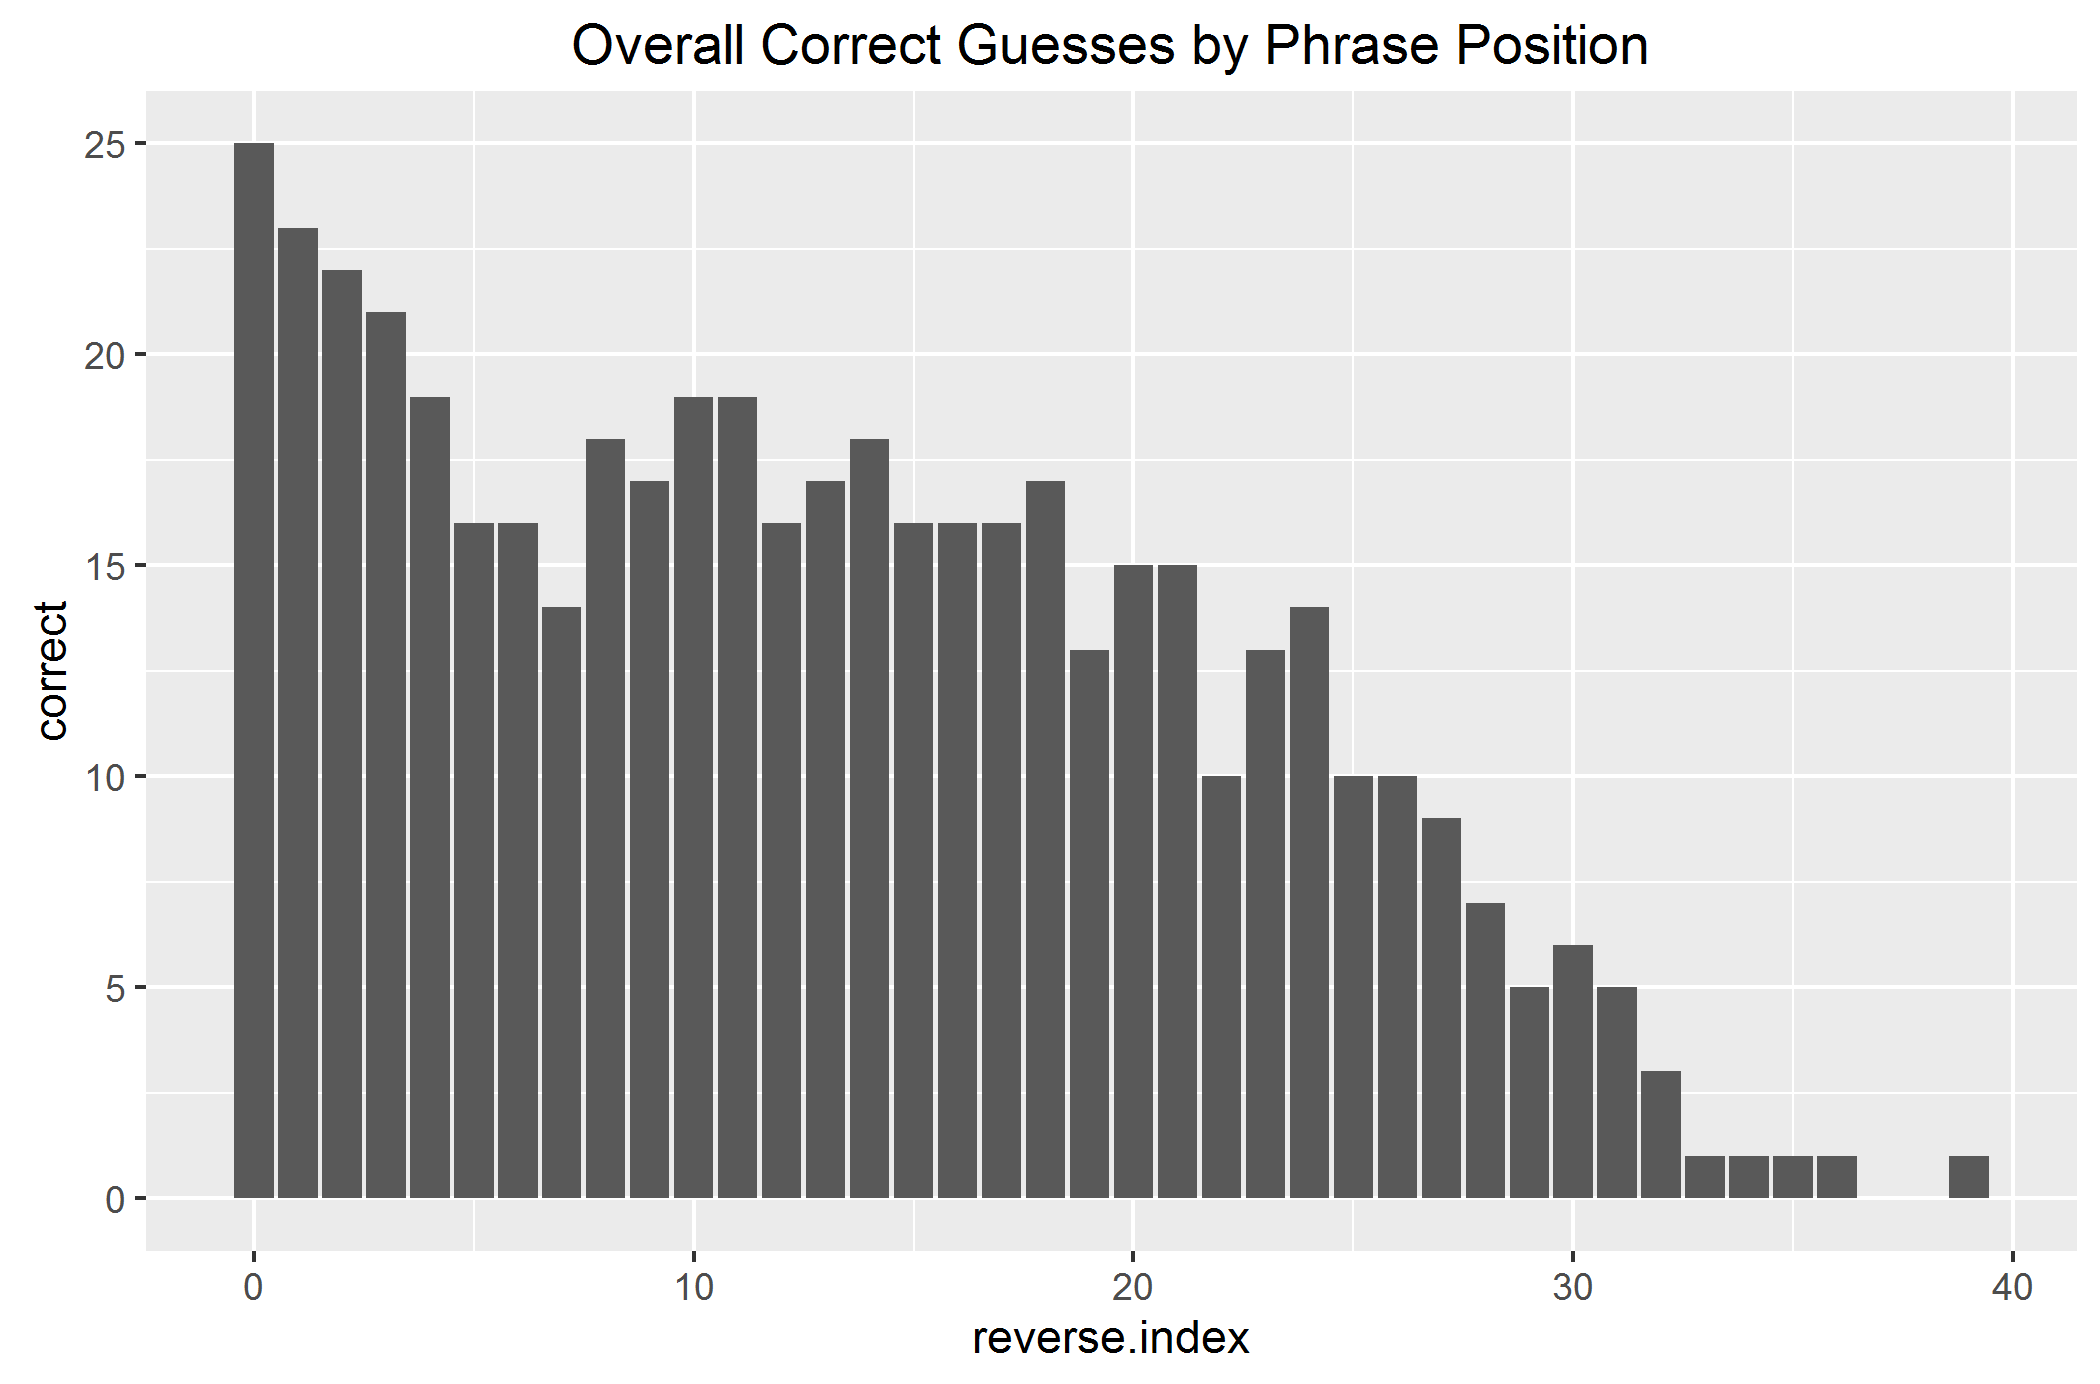
\includegraphics[width=.65\linewidth]{overall-correct-by-phrase-position}
\caption{The total correct guesses for each position in the phrase for the participant group. The index indicates the number of letters from the end of the phrase the guesses were made at. Note the undulating nature of the graph.}
\label{fig:overall-correct-by-phrase-position}
\end{figure}

\begin{figure}[h!]
\centering
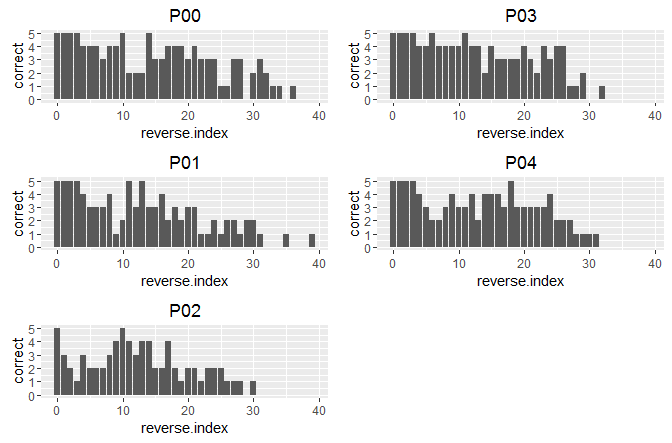
\includegraphics[width=.65\linewidth]{participant-correct-by-phrase-position}
\caption{A breakdown of correct guesses by phrase position by participants.}
\label{fig:participant-correct-by-phrase-position}
\end{figure}

Since the phrases could have different lengths, it was decided to consider the guesses by their distance from the \emph{end} of the phrase (also referred to as \emph{reverse index}). This way, phrases can be compared easier, and it seems better suited to showing the conclusion that was drawn. Overall, it is clear that participant performance improves the closer to the end of the phrase they were. In fact, you can see that every participant always guessed the last letter of the phrase correctly. It is also apparent that the ``curve" of the graph is not perfectly ``bell-curve-like" in nature; there are undulations. These undulations seem to occur near word boundaries, which will be discussed in the next section.

When we analyze the data by participant, different ``aptitude profiles" become apparent. Participant $3$ appears to have done the best at the task, with their graph almost displaying a plateau shape, with occasional spikes and valleys (likely at word boundaries). Participant $2$ appears to have the least aptitude, with a spiky graph with several peaks and valleys. The more moderate participants appear to exhibit the same peaks and valleys, but with a larger bias towards being correct.

Unfortunately, the graphs don't show it, but there is an interesting observation to be made when comparing the best performing two participants: P00 and P03. Both did well, but P03 did better. However, the graph does not show time to complete the task. When looking at the raw data, P00 took around 50 seconds per phrase. P03 took much greater care with their guesses, taking roughly twice as long (around 90 seconds per phrase). It would be interesting to compare these participants' performance if they were to use a similar amount of time to complete their guesses.

%
\subsection{Correctness By Position In Word}
\begin{figure}[h!]
\centering
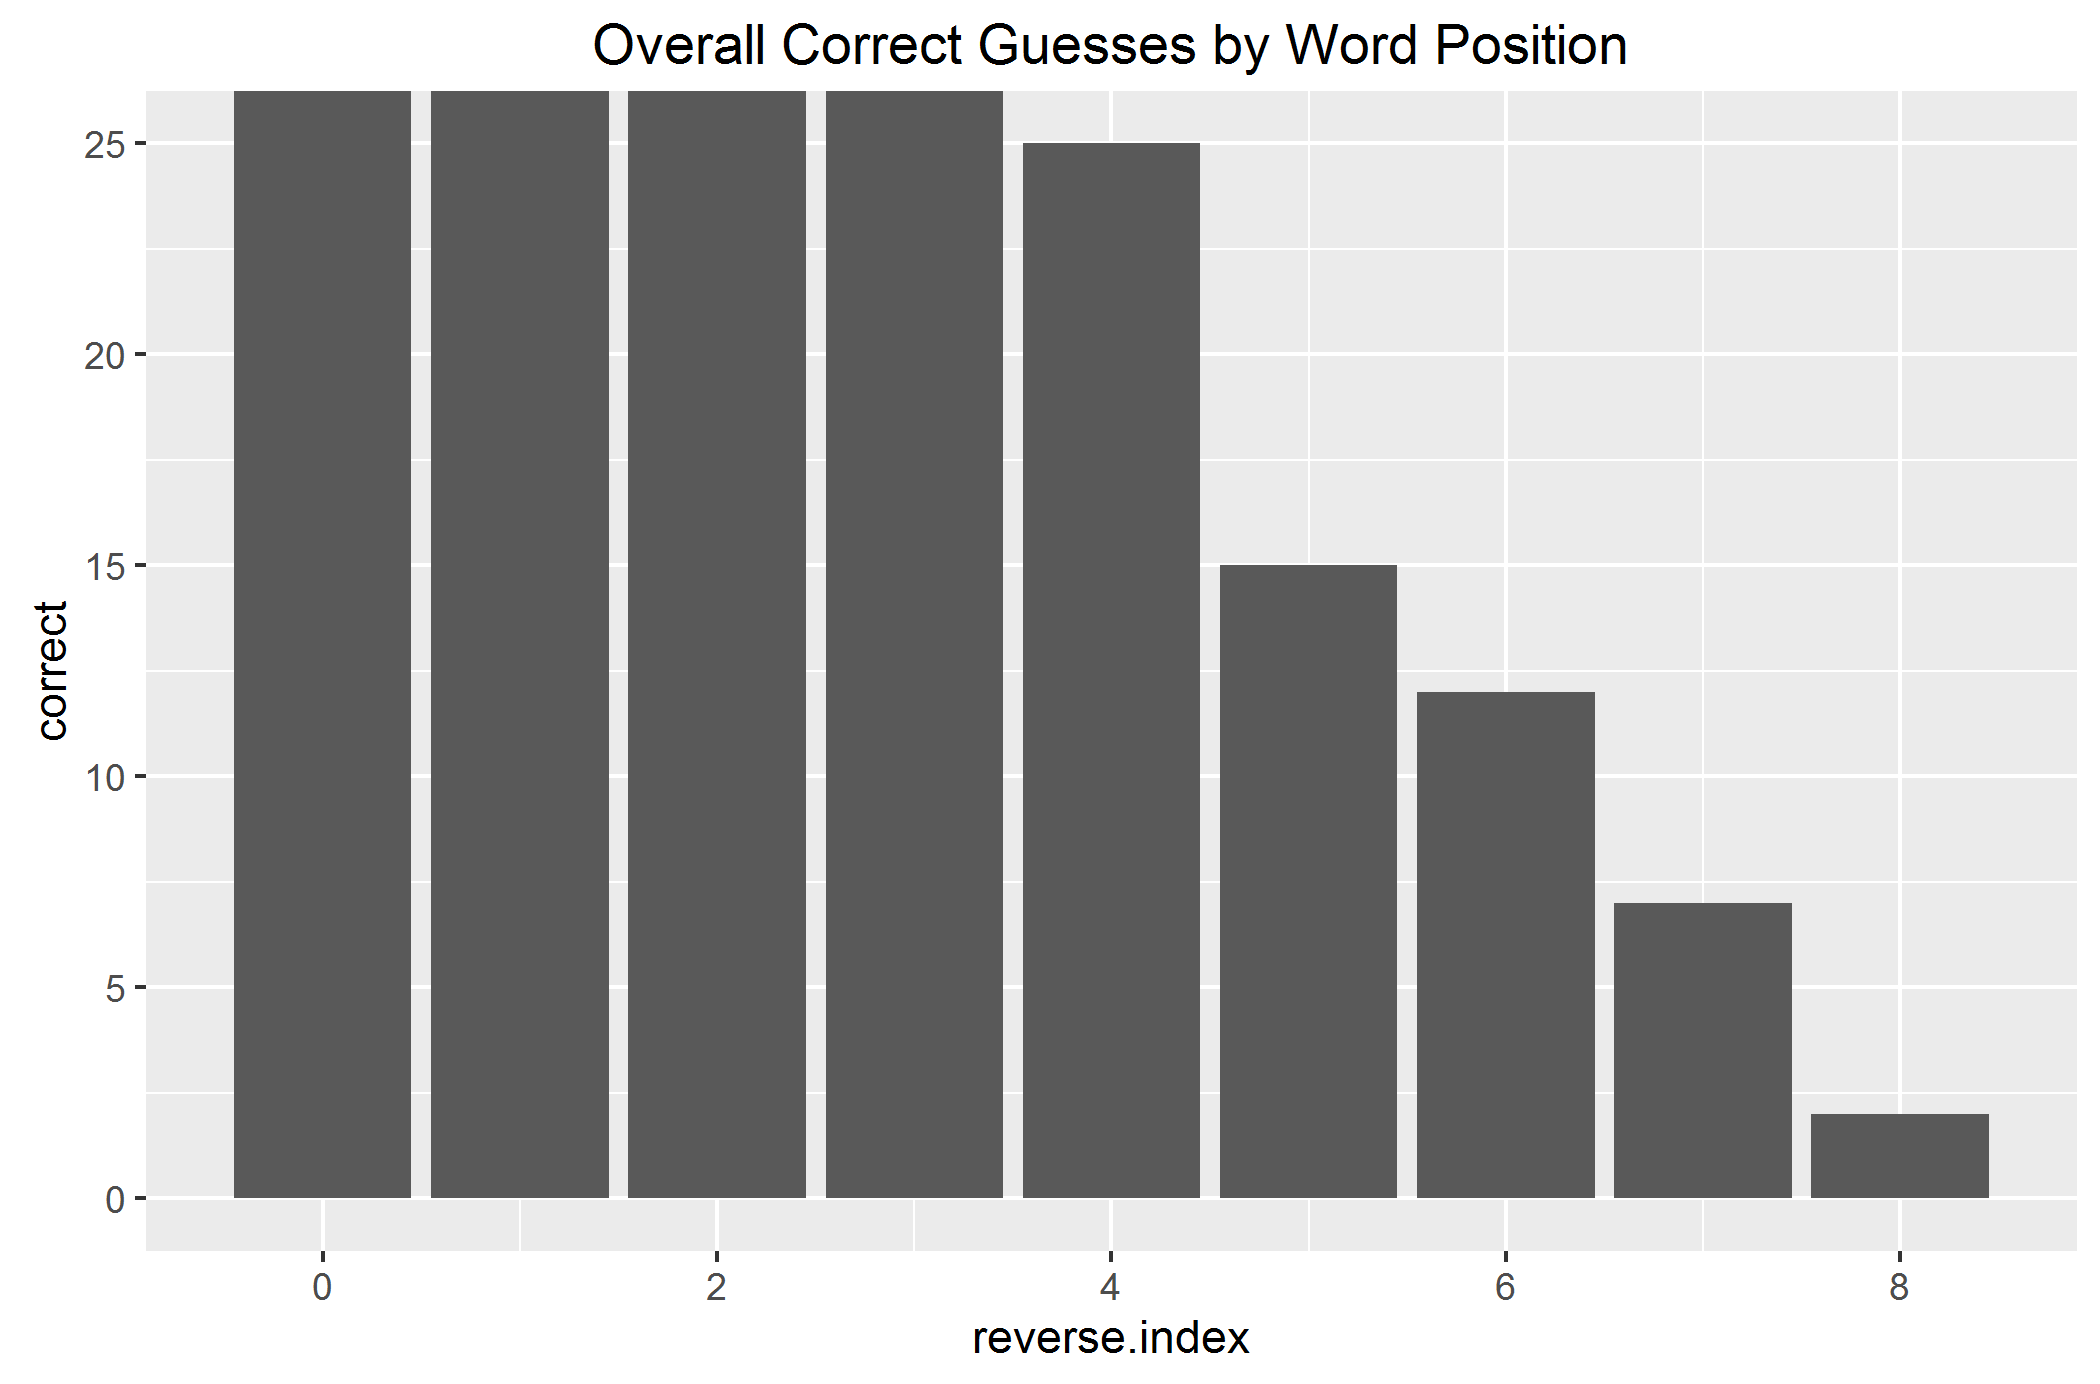
\includegraphics[width=.5\linewidth]{overall-correct-by-word-position}
\caption{The total correct guesses for each position in the word for the participant group. The index indicates the number of letters from the end of the word the guesses were made at. Guesses made where there were spaces in the phrase were not included. Note that guesses only get better the closer to the end of the word they are.}
\label{fig:overall-correct-by-word-position}
\end{figure}

\begin{figure}[h!]
\centering
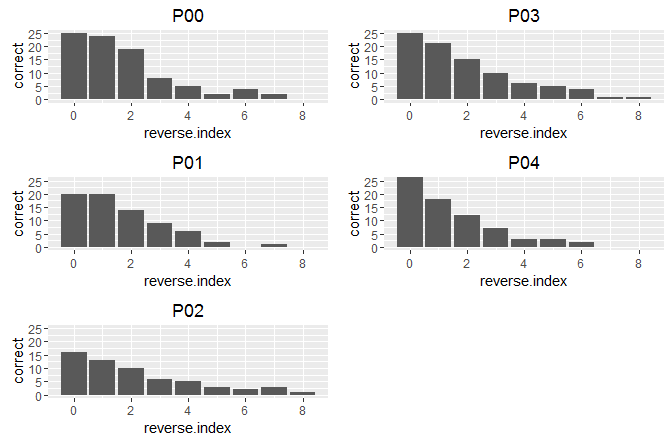
\includegraphics[width=.65\linewidth]{participant-correct-by-word-position}
\caption{A breakdown of correct guesses by word position by participants. Guesses at places where there were spaces were not included.}
\label{fig:participant-correct-by-word-position}
\end{figure}

Analyzing performance by word position (using the same indexing scheme used for the phrases - distance from the end of a word), we see the very obvious pattern of likelihood of a correct guess increasing near the end of a word. Overall, participants never did as well predicting the letter as they would on the next letter of the word.

When analyzed by participant, we see that the ``curve" of the graph is shifted more to the left and is more steep for participants with better aptitude, and is less steep for participants with less aptitude. Interestingly enough, when viewed at the participant level, we see that some of the participants actually did ``violate" the general rule that guesses closer to the end of the word were always more likely to be correct. This was likely not statistically significant and would disappear had a larger number of trials been done.

Note that for this analysis, the guesses where there were spaces between words were disregarded so as to clearly denote where a words start and end. The data would likely appear much noisier if spaces were included since participants did have difficulty predicting the end of a word. One example of such difficulty would be not knowing if a word was plural or not.

%
%
\section{Exercise 2-6}
Conduct a small experiment on human reaction time using the \texttt{ReactionTimeExperiment} software provided on this book's website. Recruit about [4+] participants. \dots Consider modifying the software in some way, such [as] using words instead of letters for the visual search task, or using an auditory stimulus instead of a visual stimulus for the simple reaction time task. The modification can serve as a point of comparison (e.g., visual search for words versus letters, or reaction time to an auditory stimulus versus a visual stimulus). Write a brief report on your findings. \\

\begin{figure}[h!]
\centering
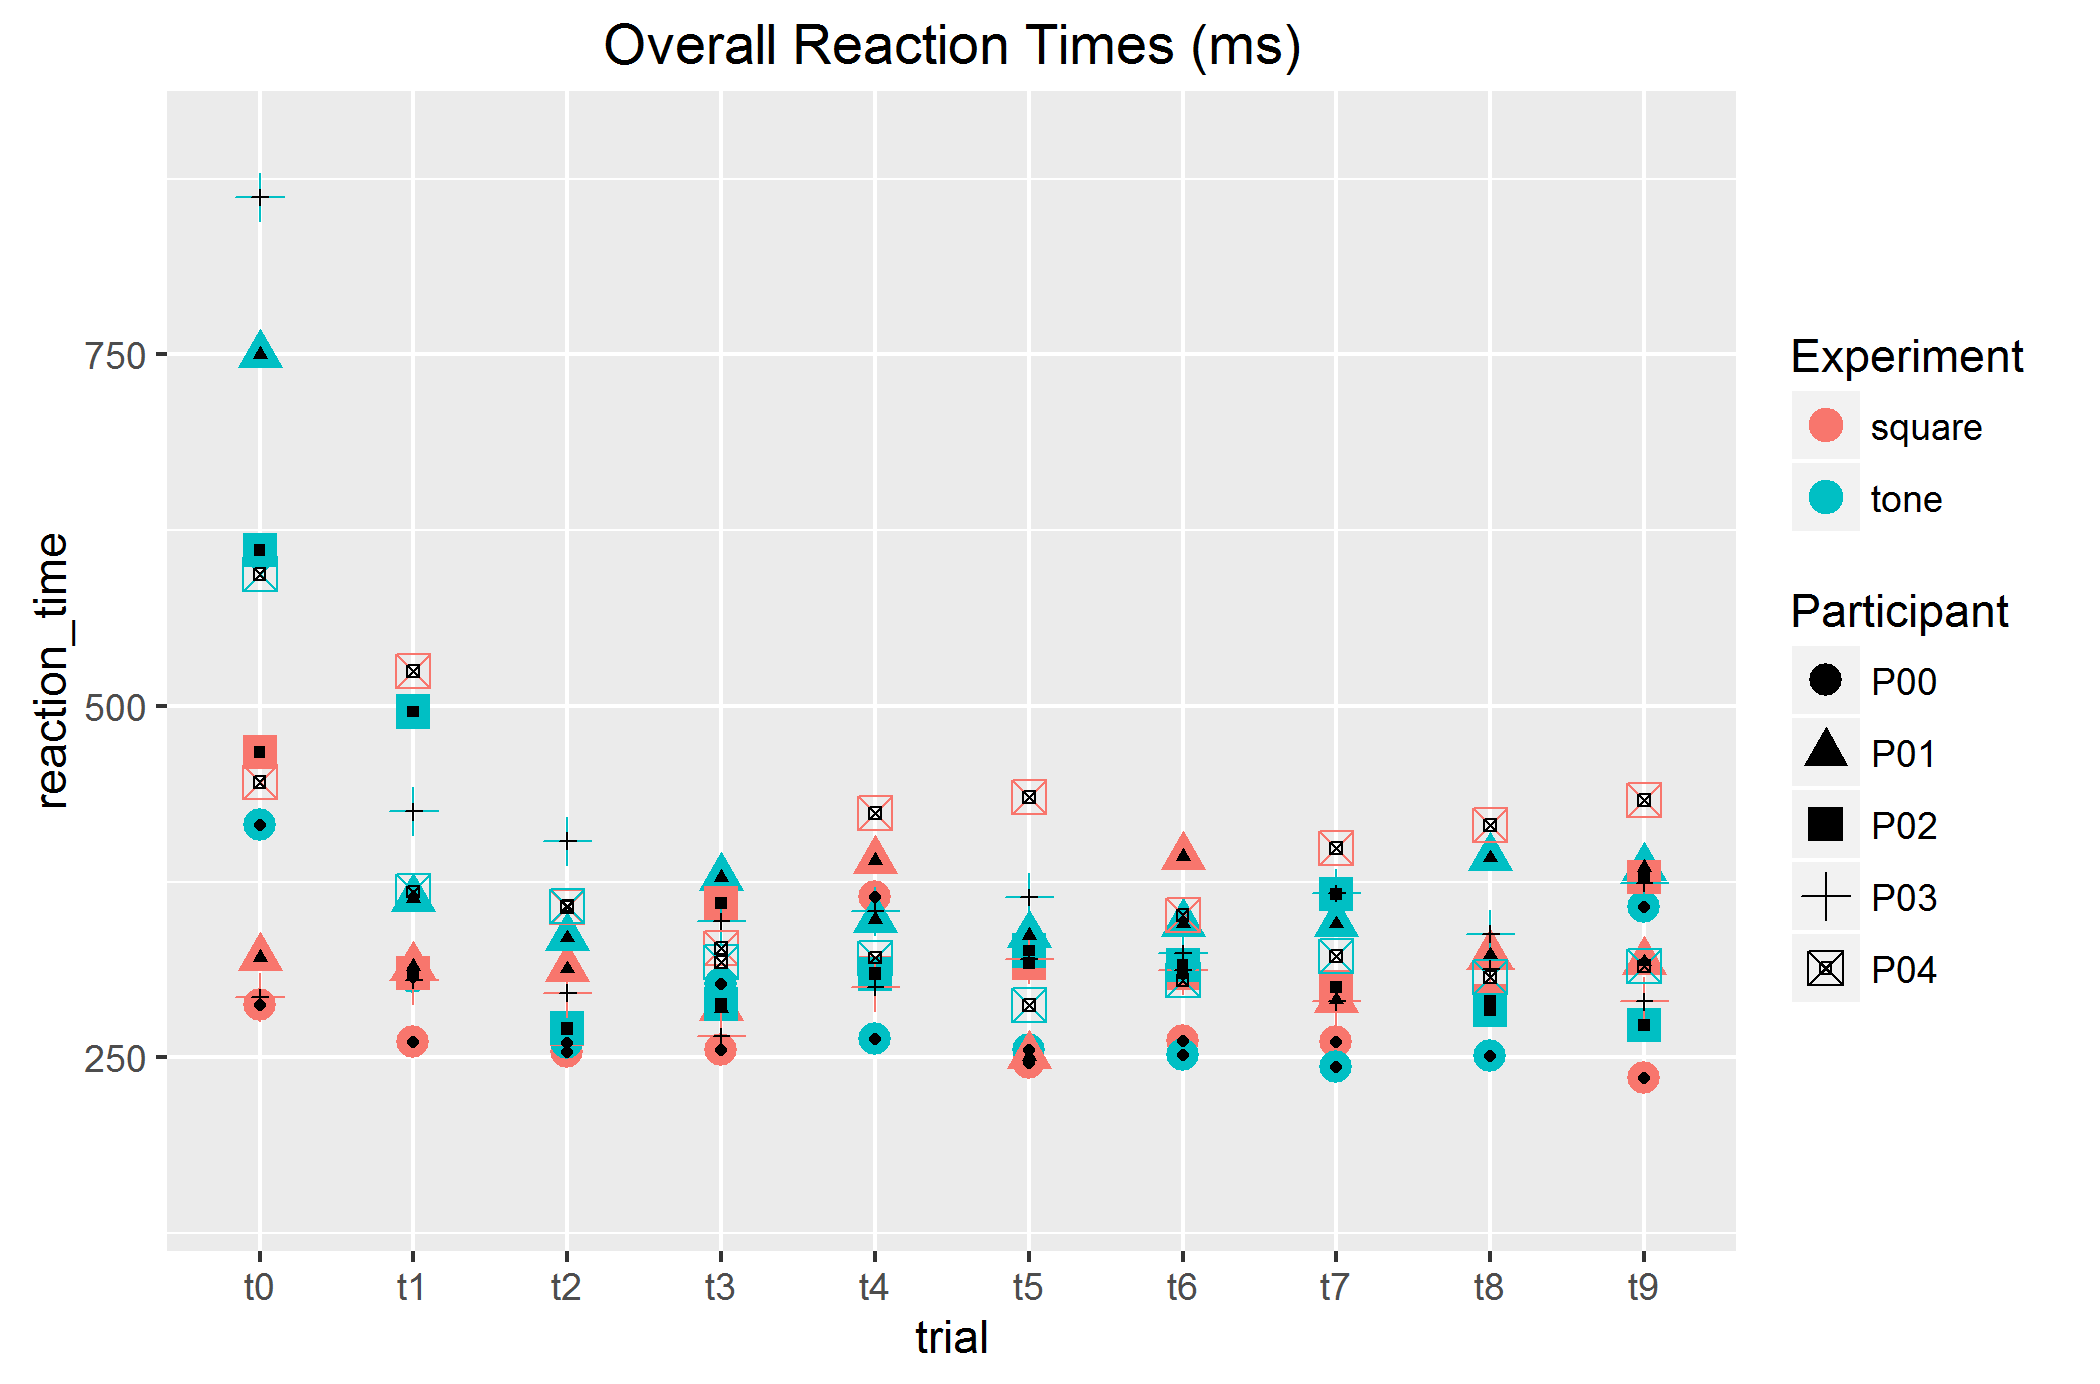
\includegraphics[width=.65\linewidth]{overall-reaction}
\caption{A scatter-plot showing the time required by each participant to react to the stimulus. Note how different stimuli affected participants differently.}
\label{fig:overall-reaction}
\end{figure}

\begin{figure}[h!]
\centering
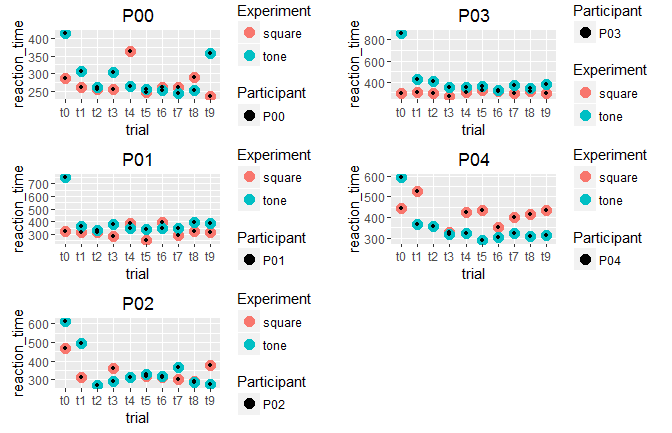
\includegraphics[width=.65\linewidth]{participant-reaction}
\caption{A breakdown of the simple reaction times by participant.}
\label{fig:participant-reaction}
\end{figure}

\subsection{Modification Made: Visual vs. Auditory Stimulus}
The experiment performed was the simple reactions test. Originally the software would change a gray square to a red one, which was the prompt for the participant to hit a key. A modification was made so that the software would play a simple tone as the stimulus to prompt the participant to press a key. The tone was the musical note $A$. Otherwise the experiment remained the same.

Both trials were performed in the same sitting for the participants; the visual trial was performed before the auditory one, although, in retrospect the could have/should have been randomized in case there was an unintended effect (such as a ``warm up" effect where participants start the second trial more ready to react than in the first).

%
\subsection{Overall Results}
In general, we can say that participants were slowest to react on the first stimulus, particularly with the auditory stimulus (although this was by no means a perfect rule). After the first stimulus, participants appeared to focus and react better. Some participants appear to have lost focus towards the middle of the experiment, regain that focus, and then lose the focus once more towards the end of the experiment.

It appears that participants were able to react under $400$ milliseconds in general, which I believe is consistent with the estimates in the chapter and generally accepted knowledge.

It is difficult to generalize about any kind of difference between the visual and auditory stimuli overall; other than the initial reactions, where participants performed better visually (perhaps the done was more difficult to initially recognize than the red square). It seems that some participants did well with one stimulus, and others performed better with the other stimulus.

%
\subsection{Participant Results}
When analyzing the data by participant, one of the easiest things to see is that it seems that participants were better at one or the other types of stimuli (participant $0$ is probably the only one that has a good mixture of ``stimulus preference"). This would support the conclusion that some stimuli are better for different users, meaning that not all interfaces work well for all users.

It is interesting to note that the participants exhibiting the highest variability (relative to their own data) were the fastest and the slowest participants (P00 and P04).

%
\subsection{Matching Results}
Since it seemed like it was too easy to just do the exercise with modified software, I did all five experiments with a subset of the original set of participants (2 of the 5). I discuss the other four experiments here. Note that a grid of size 2 was used for the visual search experiment.

\begin{figure}[h!]
\centering
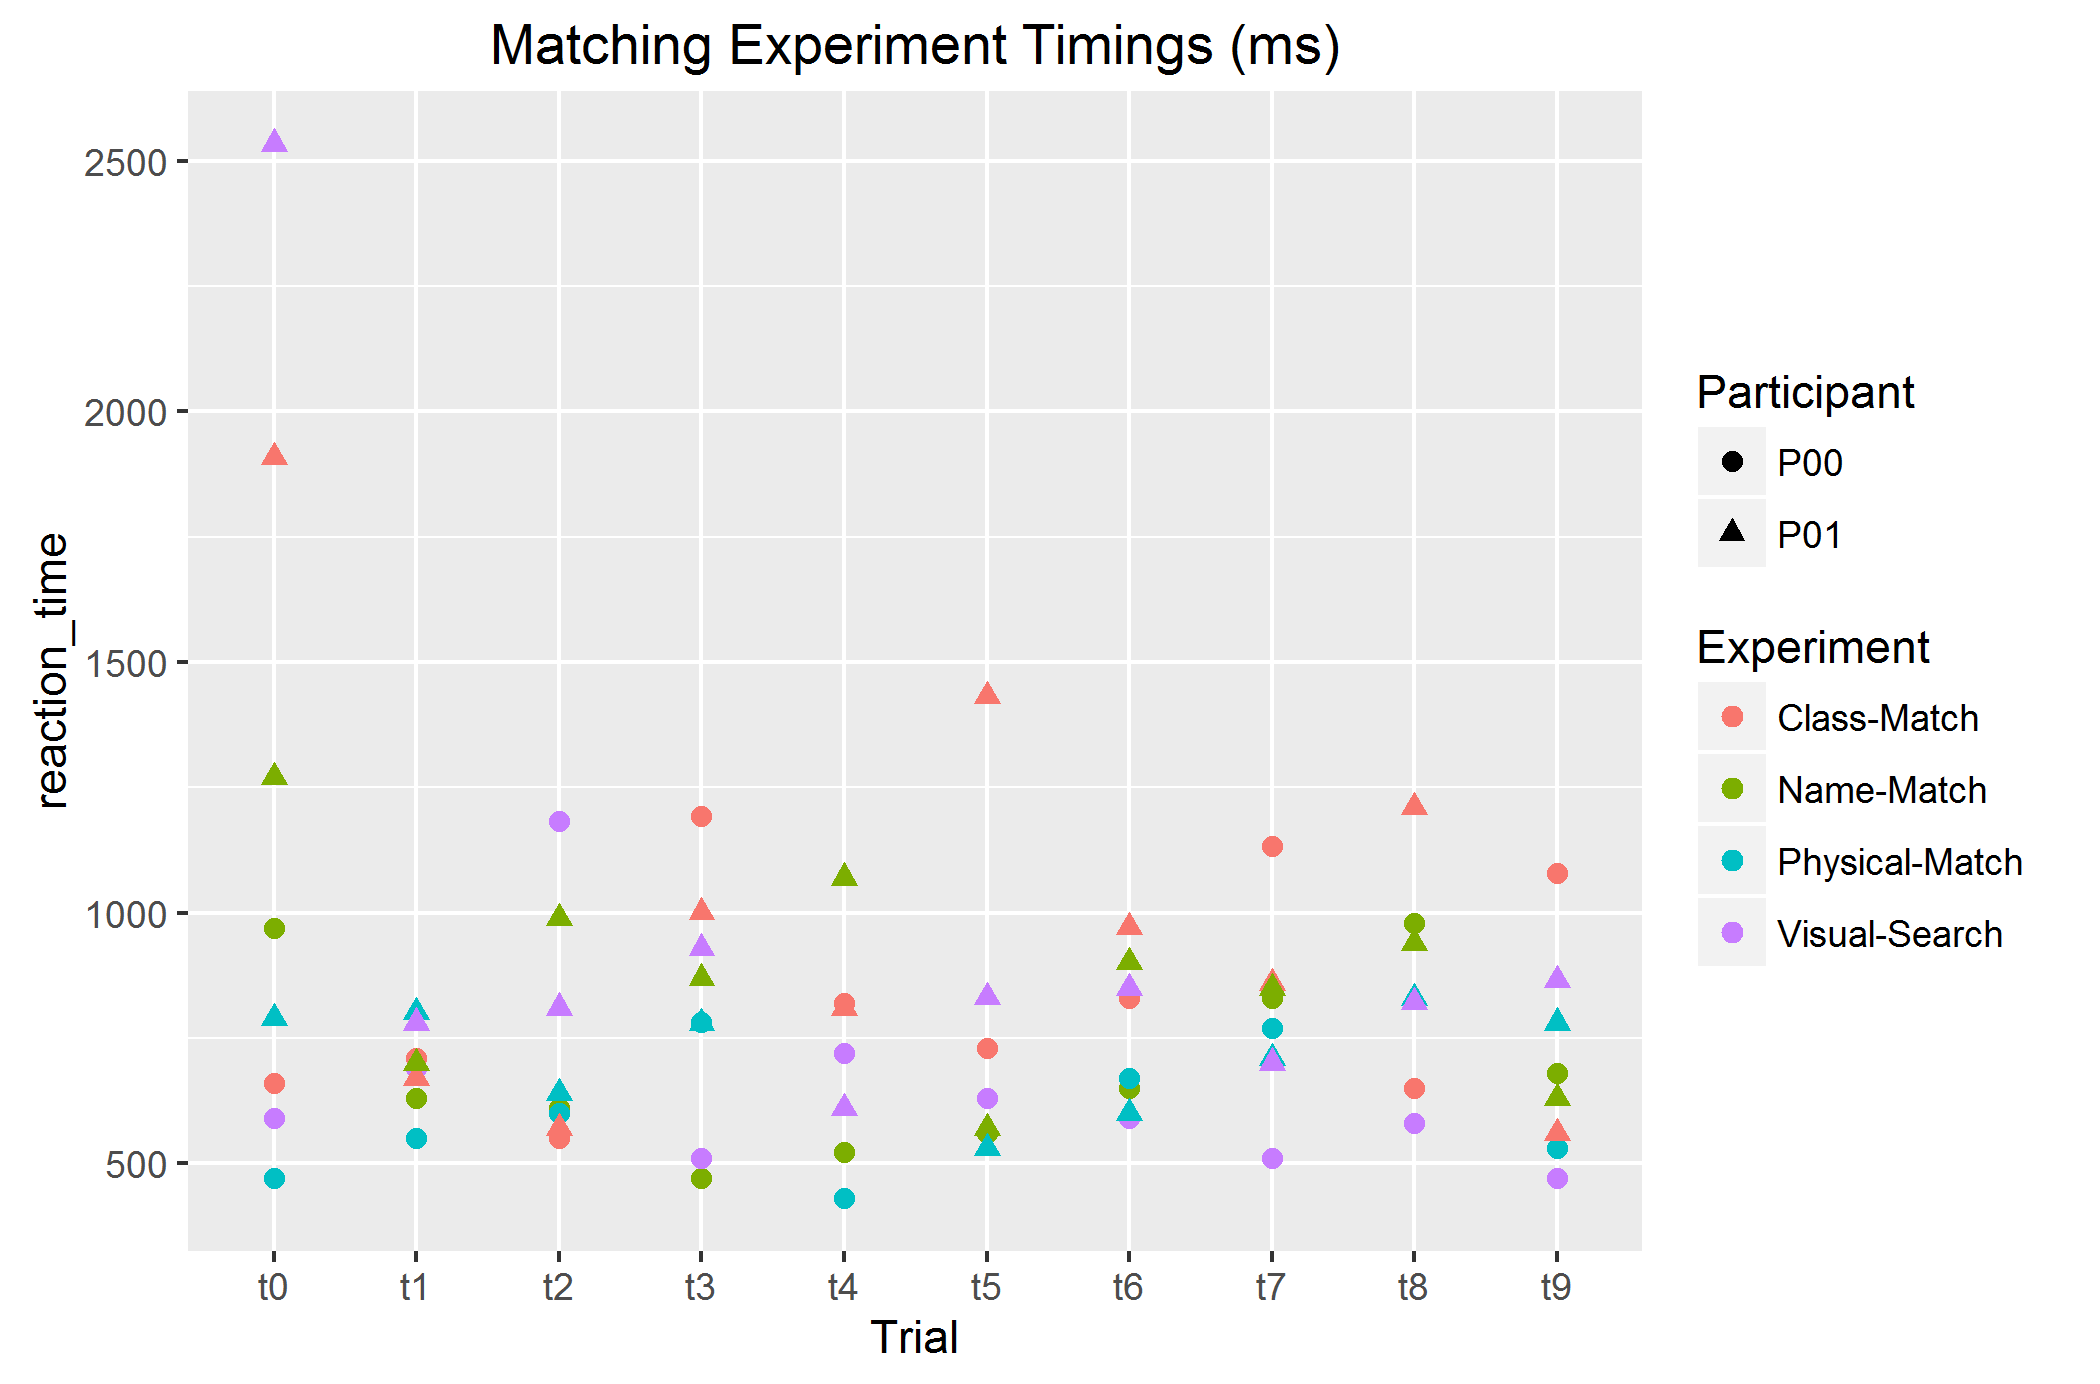
\includegraphics[width=.65\linewidth]{matching-timings}
\caption{A scatter-plot displaying the reaction times of participants for the matching reaction tasks. Note the inconsistency of time required by task now that a cognitive element has been added (compared to the simple reaction).}
\label{fig:matching-timings}
\end{figure}

\begin{figure}[h!]
\centering
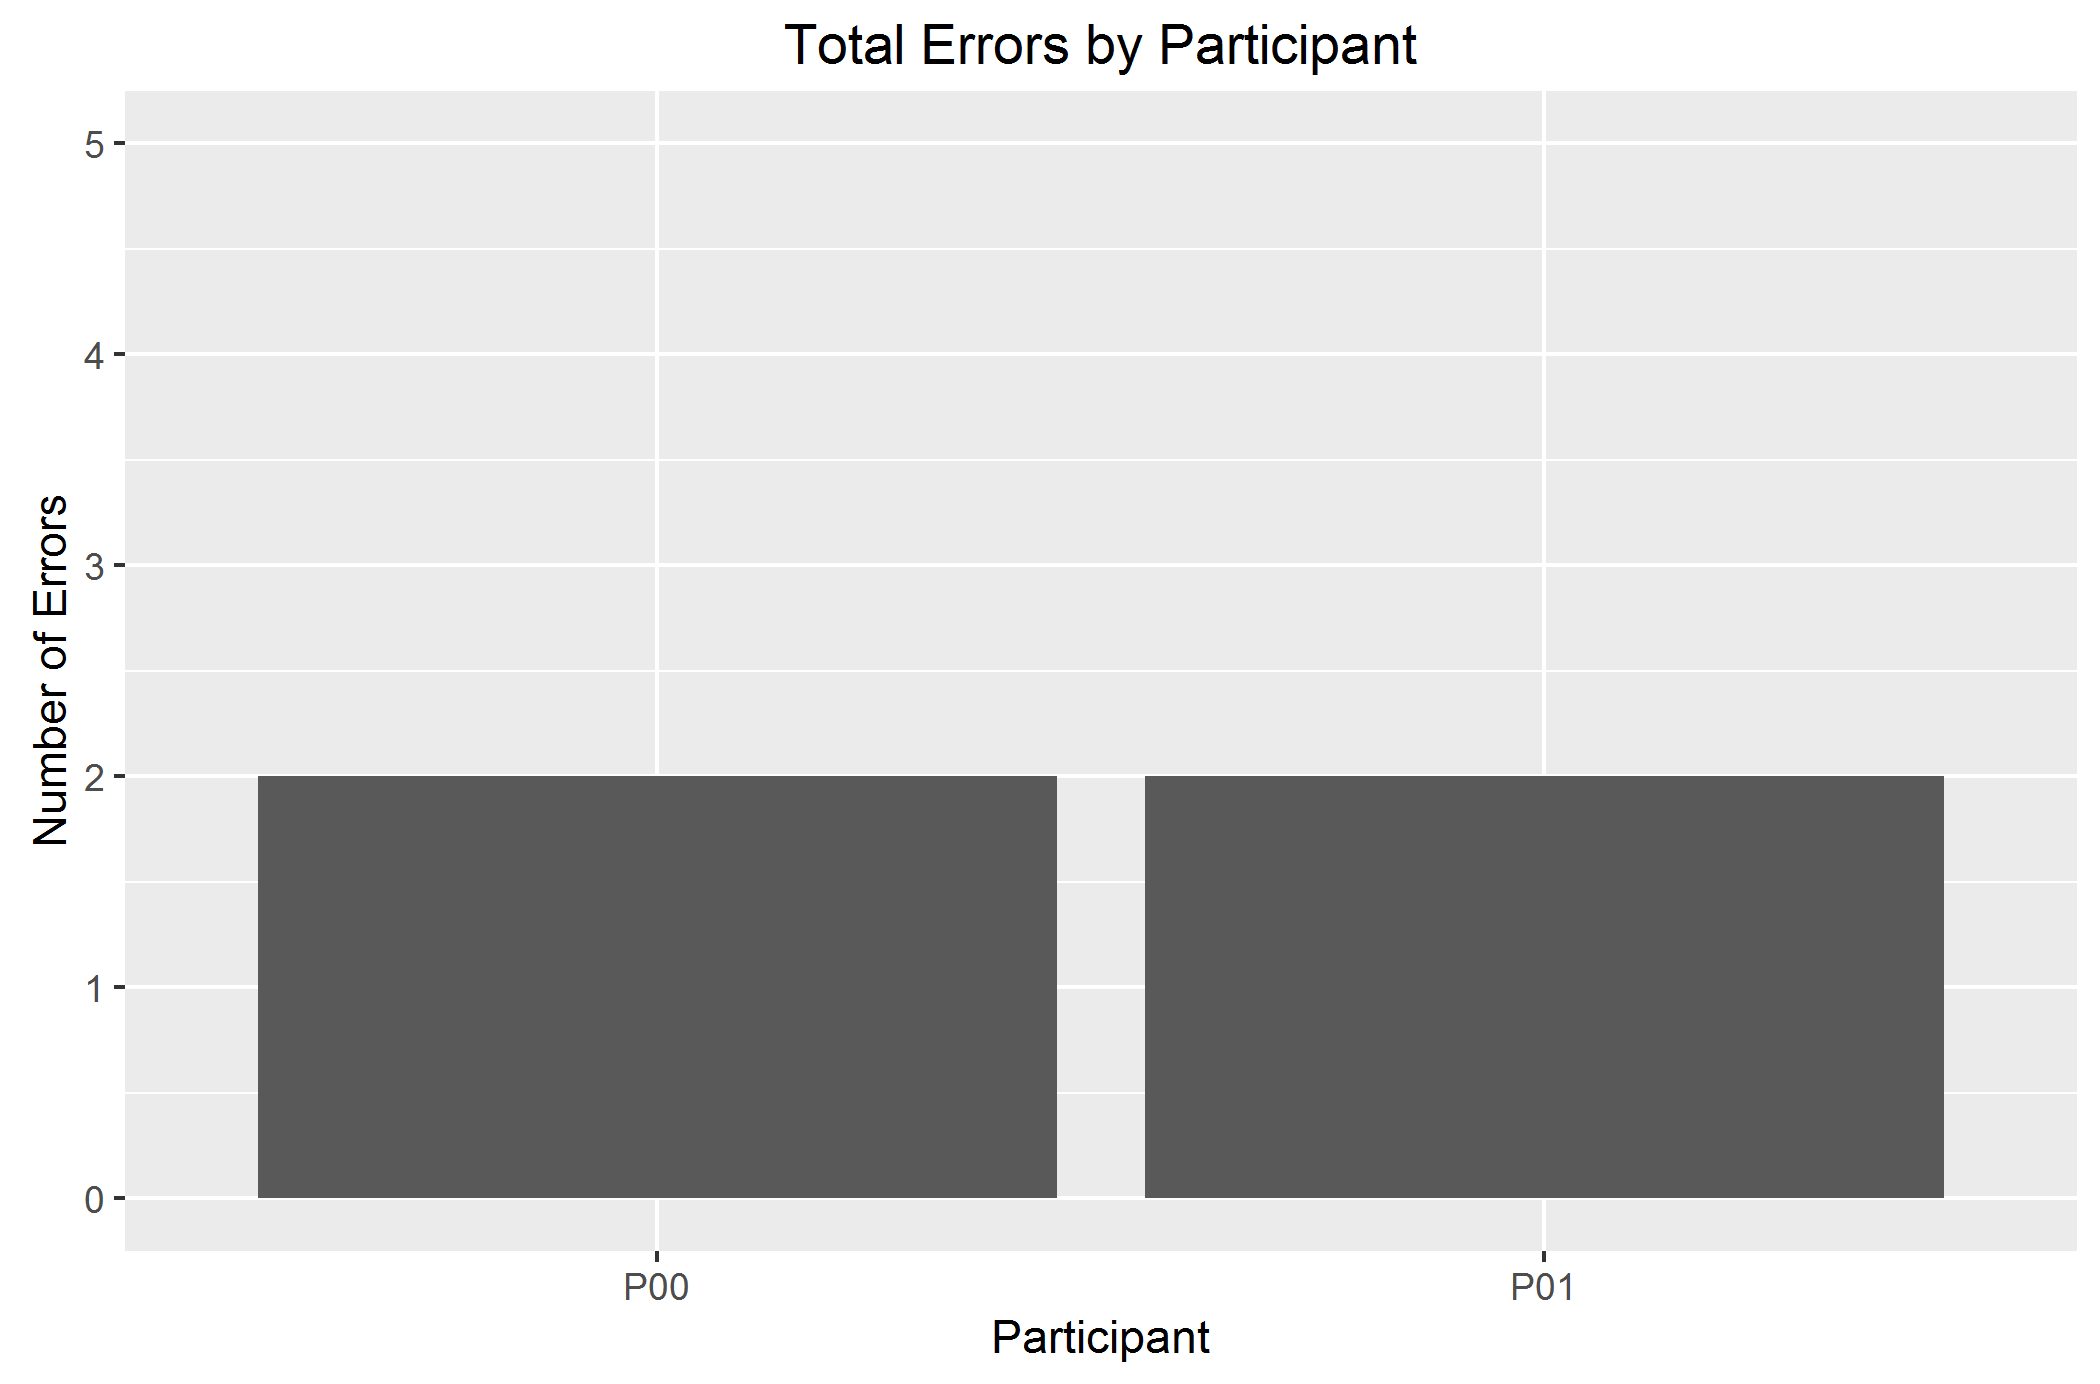
\includegraphics[width=.5\linewidth]{matching-errors}
\caption{The total numbers of errors made by participants in the matching tasks - not particularly informative.}
\label{fig:matching-errors}
\end{figure}

The matching tasks required significantly more time than the simple reaction tasks. Response times for these participants were roughly 2 to 4 times greater than in the simple reaction tasks. This is likely due to the added cognitive load of the tasks. This is roughly consistent with the time presented by the book (the book says cognitive processing should take between 70 and 300 milliseconds, the participants appear to have used 200 to 800 milliseconds more for matching tasks than simple reaction tasks).

Of the matching tasks, the class match appeared to require the most time. This is not surprising since the user has two tasks to perform instead of one: first, what are the classes of the character, letter or digit?; and second, do they match. While this might seem like fewer ``primitive operations", I think that for short words, it is fair to say that simple word equality comparison is a ``primitive operation" for the human brain.

The visual search task seems to have been completed surprisingly quickly for the participants, being one of the faster tasks. This was likely due to the small grid used, and this task would likely become dramatically slower as the size of the grid increases.

Unfortunately, we cannot make meaningful generalizations from the number of errors made by the participants. They only made 2 each, with both errors being in different experiments. Not only do the participants not really differ, this is just too few errors to really say anything with any significance other than ``the participants occasionally made errors". More and longer trials might produce meaningful results.

%
\end{document}
